\documentclass[15pt,margin=1in,innermargin=-4.5in,blockverticalspace=-0.25in]{tikzposter}
\geometry{paperwidth=42in,paperheight=30in}
\usepackage[utf8]{inputenc}
\usepackage{amsmath}
\usepackage{amsfonts}
\usepackage{amsthm}
\usepackage{amssymb}
\usepackage{mathrsfs}
\usepackage{graphicx}
\usepackage{adjustbox}
\usepackage{enumitem}
\usepackage[backend=biber,style=numeric]{biblatex}
\usepackage{emory-theme}
\renewcommand{\familydefault}{\sfdefault}

\usepackage{mwe} % for placeholder images

\addbibresource{refs.bib}

% set theme parameters
\tikzposterlatexaffectionproofoff
\usetheme{EmoryTheme}
\usecolorstyle{EmoryStyle}

\title{Reproduction of `Multi-Task Learning using Uncertainty to Weigh Losses'}
\author{D. Baerg, O. Key, J. Materzynska and M. Tong}
\institute{Department of Computer Science, University of Oxford}
%\titlegraphic{\includegraphics[width=0.07\textwidth]{Emory_vt_280.png}}

% begin document
\begin{document}
\maketitle


\centering
\begin{columns}
    \column{0.32}
    
    \block{}{
        
        We reproduced a selection of experiments from `Multi-Task Learning using Uncertainty to Weigh Losses'\textsuperscript{\cite{KendallGalCipolla2017Multi}}. This paper makes a new approach to multi-task learning by using aleatoric homoscedastic uncertainty to weigh losses in different tasks. They used a `unified' architecture with the same encoder for different tasks, with only the decoder differing between tasks. This allowed them to achieve a better performance with multi-task learning than with multiple single-task learning.
    }
    \block{Background}{
        Background on multi-task learning.
        
    }
    \block{Objective}{
       We aimed to reproduce the results comparing multi-task learning with single-task learning with the sub-sampled version of the Cityscapes dataset\textsuperscript{\cite{Cityscapes}}, Tiny Cityscapes.
       
       \begin{tikzfigure}[Results that we aimed to reproduce\textsuperscript{\cite{KendallGalCipolla2017Multi}}]
            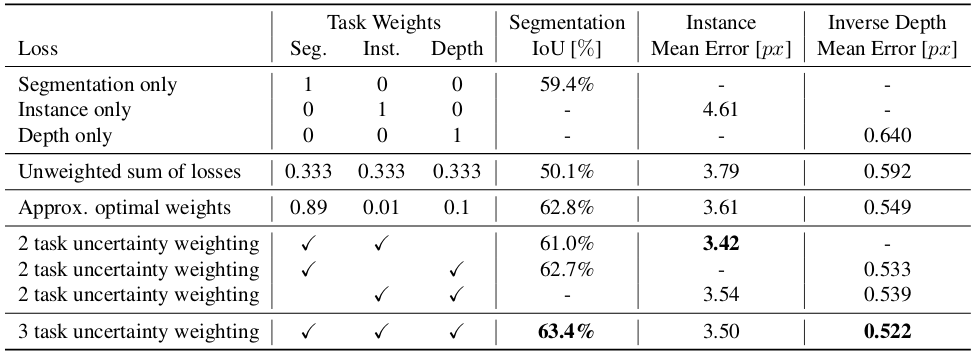
\includegraphics[width=1\linewidth]{data.png}
        \end{tikzfigure}
        
    }
    \block{Method}{
        
        We reproduced the method given in the paper in PyTorch with four main differences:
        \begin{itemize}
         \item Training set: $32 \times 32$ crops of Tiny Cityscapes training set images.
         \item Validation set: $128 \times 256$ Tiny Cityscapes validation set images.
         \item Optimiser: Adam with default parameters\textsuperscript{\cite{Adam}}.
         \item Clustering algorithm: DBSCAN.
         \end{itemize}
         
         We used ResNet\textsuperscript{\cite{ResNet}} and DeepLab\textsuperscript{\cite{DeepLabv3}\cite{DeepLab}} papers as reference for the encoder architecture.
         
        We also were not able to use the depth data.
        
        
    }
    \column{0.36}
    \block{Results}{
         Our results
    }

    \column{0.32}
    \block{Comparison}{
        How our results compare with their results
        }
    
    \block{Summary}{
        
    }
    
    \block{References}{
        \vspace{-1em}
        \begin{footnotesize}
        \printbibliography[heading=none]
        \end{footnotesize}
    }
\end{columns}
\end{document}